%! TEX root = 'main.tex'

%\section{Experiments}

\section{Implementation}
\label{sec:implementation}

In this section, we give some implementation details and issues that we had during development.

\subsection{Hypervisor}


There are two new modes to run under virtualization: VMX root operation and VMX non-root operation. VMX stands for virtual machine extension. It proves new instructions VMXON, VMXOFF, VMPTRLD, VMPTRST, VMCLEAR, VMREAD, VMWRITE, VMCALL, VMLAUNCH, VMRESUME.

Usually processor has running mode known as ring-0 to ring-3, where ring-0 is kernel mode, ring-3 is user mode, ring 1 and ring 2 are rarely used. When CPU enables virtualization, it could be seen as running in the non-root mode. The root mode can be considered as a lower and more privileged level, it controls the whole CPU. And the guest operating system will run in non-root mode. Root mode runs VMM (Virtual Machine Monitor) is often called ring -1.

VMXON and VMXOFF are instructions to enter and exit VMX mode. There is an important data structure called VMCS (Virtual-Machine Control Structure), which is 4 KB large in size. It controls the state switch between VMX root mode and VMX non-root mode. From root mode to non-root mode called VM Exit. From non-root mode to root mode called VM Enter.

Every logical CPU (each core in a real physical CPU is called a logical CPU) has a processor state called VMCS pointer. It contains the physical address of the VMCS. There could be many VMCSs, the one stored in VMCS pointer is considered as the current one. Every VMCS can represent a virtual processor for the virtual machine, inside virtual machine, that is a logical CPU seen by operating system. Although hypervisor knows the physical address of a VMCS, but hypervisor cannot modify it directly, hypervisor can only reads and writes VMCS using VMREAD, VMWRITE instructions. Hypervisor use VMPTRLD to set a VMCS both as active and current. And use VMCLEAR to mark the VMCS as inactive.

A VMCS contains many fields related every aspect of a virtual machine. There are six fields: Guest-state area, Host-state area, VM-execution control fields, VM-exit control fields, VM-entry control fields and VM-exit information fields. And each field also contains many more control fields with a lot of settings. Once the CPU enters into a virtual machine by execute VMLAUNCH which associates with a VMCS, this virtual machine is fully control by the settings in the VMCS. For example, the CR4 field in the Guest-state area is the one we used to update the actual CPU register.  Hypervisor can set during what circumstances the virtual machine should exit. And then the hypervisor can handle this situation, for example emulate a hardware device or change the virtual machine's behavior. In this case, it's the control register related operations that we are interested. 

We do not actually emulate any hardware device, we put the current system into a virtual machine environment and our code run as the hypervisor.

\subsection{Page Faults}
Handling exceptions is the major part of this mitigation. The type we need to handle is page fault exception. They may be caused directly by SMAP or by our protection on the pages. Even though it's called "page fault", but not all exceptions are due to program errors. For example, page fault is one part of paging mechanism in x86 architecture to make the virtual memory much larger then the physical memory that exists in the system. 

We need to handle all the page fault exceptions before the system's handler does. Some of the them need to be passed to the operating system, for example, those invalid pages. And the others need to be intercepted. There is a 32-bit error code being pushed into the kernel stack when exception triggered, as shown in~\autoref{fig:pagefaulterrorcode}.


\begin{figure}[th]
  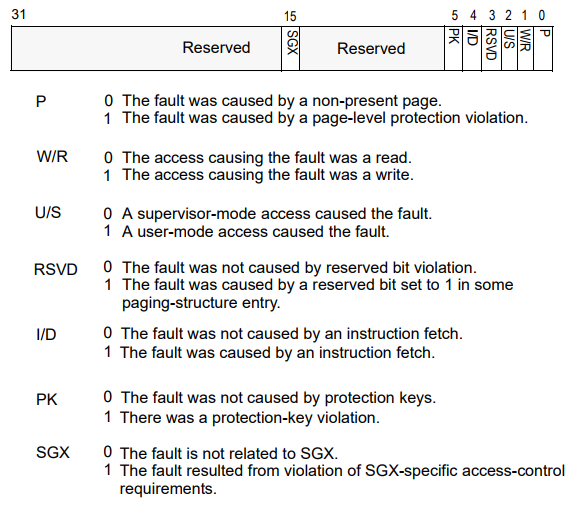
\includegraphics[width=0.47\textwidth]{figures/pagefaulterrorcode}
  \centering
  \caption{Page Fault Error Code.~\cite{intelinterrupt} Unfortunately, SMAP doesn't have a separate bit. The exception it triggers comes with U/S bit set to 0, but the reason for that is not unique.}
  \label{fig:pagefaulterrorcode}
\end{figure}

The bits don't clearly indicate the cause. For example, there is no "SMAP" bit. So our page fault handler needs to collect more information in order to tell the possible reason for the exception. Register values of EIP, CS, ESP, SS, EFLAGS are also pushed into the kernel stack with the error code. We also get the page table root from CR3 and the faulting virtual address from CR2.

First, We need to screen out some of the cases that are irrelevant. For example, When exceptions come in with "P" bit unset, indicating that the page is not present in the memory. It's part of the paging mechanism, pages can be swapped out to secondary storage such as hard disk. Even our page fault handler itself may trigger this type of page faults. Since page tables are reside in the page-able pages, so when we walk through the page table, some of the PTE pages may not be there. Therefore we need to pass such page faults to operating system as soon as possible, otherwise it will cause a dead loop inside our handler. We also observe that there is no exception caused both by non-present page and SMAP at the same time, so it's safe to do so.

After screen out unrelated exceptions, the algorithm that handles mitigation related exceptions is shown in Algorithm~\ref{algo:pagefaulthandler}.


\begin{algorithm}[ht]
\begin{algorithmic}[1]
\small
\Procedure{PageFaultHandler}{}

\State $address\gets cr2$ 
\State $pte\gets \Call{\textbf{GET\_PTE}}{address}$
\State $teb\gets fs:0x18$

\If{$smap\_violation$}
	\State $pages[]\gets \Call{\textbf{ADD\_PAGE}}{$address, pte, cr3, teb$}$
    \State $\Call{\textbf{SET\_PAGE\_KERNEL}}{pte}$
    \State $\Call{\textbf{Flush\_TLB}}{address}$
    \State \Return{$re-execute$}
\ElsIf{$user\_access\_protected\_page$}
	\If{$error.WRITE$}
    	\Repeat 
        \State{$\Call{\textbf{SLEEP}}$}
        \If{$\Call{\textbf{Check\_Permits}}{pte}$}
        	\State \Return{$re-execute$}
        \EndIf
        \Until{$count < 10$}
        \State \Return{$terminate\_thread$}
    \Else
    	\State $\Call{\textbf{SET\_PAGE\_USER\_READONLY}}{pte}$
    	\State $\Call{\textbf{Flush\_TLB}}{address}$
        \State \Return{$re-execute$}
    \EndIf
%\ElsIf{$user\_write\_readonlypage$}
%	\If{\Call{HAS\_RECORD}{pte}}
%    \EndIf
\EndIf
\State \Return{$original\_handler$}
   
\EndProcedure
\end{algorithmic}
\normalsize
\caption{Page Fault Handler}
\label{algo:pagefaulthandler}
\end{algorithm}


Another technical detail we should mention is that when entering page fault handler, interrupts are tuned off automatically. This is because exception is raised through an "interrupt gate". The CPU clears the IF(Interrupt enable flag) in the EFLAGS register and sets it back when interrupts return. In our case, after getting the faulting virtual address from CR2, we immediately set the IF flag by executing instruction "STI" in order to let the processor being able to receive nested exceptions.

\subsection{PTE Update}

After getting the right exception, we need to change bits of the corresponding PTE as we mentioned earlier. In a multi-processor system, updating global data such as page tables need to hold a global lock to synchronize. Since Windows operating system doesn't open such interface to third-party drivers, we can only synchronize our own operations. Because in a attacking scenario, there will be at least two threads, one is calling the vulnerable system service and the other is modifying the data. They repeat themselves in high frequency to win the race. Therefore, the page fault handler will get the corresponding exceptions also in high frequency. 

As shown in~\autoref{fig:pte}, U/S bit controls whether the page is a user page or a kernel page. R/W is the Read/Write permissions flag. The data structure of PTE on 32-bit system defined as following:
%frame=single, 
\begin{lstlisting}[basicstyle=\small] 
typedef struct _PTE_HARDWARE
{
	ULONG Valid : 1;
	ULONG Write : 1;
	ULONG Owner : 1;
	ULONG WriteThrough : 1;
	ULONG CacheDisable : 1;
	ULONG Accessed : 1;
	ULONG Dirty : 1;
	ULONG Reserved : 1;
	ULONG Global : 1;
	ULONG Ignored: 3;
	ULONG PageFrameNumber : 20;
} PTE_HARDWARE, *PPTE_HARDWARE;

typedef struct _PTE {
	union {
		ULONG Long;
		PTE_HARDWARE Hard;
	} u;
} PTE, *PPTE;
\end{lstlisting}


C code that update one bit of a PTE, such as the following:

\begin{lstlisting}[basicstyle=\small] 
pPte->u.Hard.Owner = 0;
\end{lstlisting}

%Such C code normally would be translated into assembly like the following.
Where pPte is a PTE pointer. Such simple code has concurrency issue. It's assembly code is listed as the following:

\begin{lstlisting}[basicstyle=\small] 
1) mov eax, dword ptr [pPte]
2) mov ecx, dword ptr [eax]
3) and ecx, 0FFFFFFFBh
4) mov dword ptr [eax], ecx
\end{lstlisting}

It shows that compiler generated assembly code needs three operations to update a bit that locates in the memory. First, read memory into a register; second, bit operation on the register; then write the register back to memory.

Suppose another thread at the same time try to update the same memory location but a different bit (with slightly different mask in step 3). Thread A first executes at step 3 where the memory value has been read into ecx and then updated by the "and" operation. Meanwhile, thread B executes at step 2 where the ecx register holds the old value. Next, thread A executes at step 4 and write the memory with the updated value. Then thread B executes at step 3 and step 4, writing an out dated value into memory.

To solve this concurrency issue, we can choose either using spinlocks to synchronize all the PTE operations that we make or atomic bit operation instructions.

Intel processor supports locked atomic operations on memory locations. One of the mechanism is bus locking which use of LOCK instruction prefix~\cite{intelmanualchapter8}. For example, to set/unset R/W and U/K bits in a PTE, we can use the following instructions.

\begin{lstlisting}[basicstyle=\small] 
mov eax, 'addr'
lock or/and [eax], 'mask'
\end{lstlisting}

\subsection{TLB Flushing}
A TLB(Translation Lookaside Buffer) is a memory cache that is used to store the mappings between virtual pages and physical pages as well as page attributes, in order to reduce the time taken to walk through the page tables that locate in memory, which is slower compares to cache. 

Different than data cache, TLB is not entirely transparent to the operating system. When operating system updates page tables, related TLB entries need to be invalidated. Since our solution rely upon page permits, we need to invalidate the corresponding TLB entries to make new page permits effective.

To invalidate one particular TLB entry, using instruction "INVLPG" with a source operand which is a virtual memory address. The processor determines the page that contains that address and flushes the TLB entry. INVLPG only invalidate TLB entries on the current processor. On SMP system, since many threads in one process could be scheduled on different processors, more then one processor could have the same TLB entry in their cache. To invalidate all of them, we need to issue an IPI(Inter-Processor Interruption) in order to inform all the related processors in the system.

IPI allows a processor to send interrupt signals to other processors. It's different than normal "interrupt" which go through an IRQ line. IPI signal needs to be sent via the APIC (Advanced Programmable Interrupt Controller) bus which connects all the local APIC of each processor.

In our implementation, we reuse some of the functionality from Windows operating system to issue such an IPI packet that indicate a TLB flushing to all the related processors, except the current one which is issuing the IPI.

\subsection{Crashing Thread}

As mentioned earlier, to solve the problem that a user mode thread tries to write a protected page, instead of crashing the thread immediately, our approach is to hold the thread for some milliseconds waiting for the function to end. To avoid any deadlock or blockage caused by a faulty program, the retries are only allowed for several times. 

Since it's troublesome to call undocumented functions to handle exceptions. We choose to let the operating system terminating it. We clears "p" bit of the corresponding PTE as well as changing the error code to a value that indicates "accessing an invalid page" instead of "writing an read-only page". This is because when we passing the exception to the original page fault handler, the PTE's attributes could be changed during this short period of time by another thread triggering SMAP exceptions, especially in an attacking scenario. 


%global hook, it may use shared memory,  before put it here, probably should figure out how page permits works on shared page


\subsection{Special Cases}
We assume 32bit Windows operating system use the default 2G/2G user/kernel split where user space is below 0x7FFFFFFF. More precisely, a kernel variable MmUserProbeAddress contains the highest possible address for user data, which is set to 0x7FFF0000. And we learn that one page locates at 0x7FFE0000 is defined as USER\_SHARED\_DATA. It's a shared page between user mode and kernel mode, meaning the same physical page is mapped both at 0x7FFE0000 and 0xFFDF0000. It's a read-only page and contains a lot of process settings such as system time. Kernel needs to read this page a lot. We treat such page specially to further improve performance. 


\subsection{Evaluation}

In this section, we evaluates our project's performance overhead and how it's protecting operating system from real-world vulnerabilities.

All experiments are preformed on the desktop which has Intel Core I5-6400 (6 GEN CPU Skylake), ASUS H110M-C mother board(Intel H110 Chipset, Realtek RTL8111H Network Controller), 8GB ram and 500GB hard disk.

CVE-2008-2252 is a typical TOCTOU vulnerability which is analyzed as a example in many previous researches. To evaluate the effectiveness of our mitigation, We tested it on a desktop with Windows XP installed. It's troublesome to install an old Windows operating system on a modern PC, particularly, because modern chipset which integrated hard disk controller no longer support IDE mode. Hence we need ASUS AHCI driver for Windows XP, tool that can make a USB stick bootable and tool that virtualize a floppy drive~\cite{installxpskylake} for providing AHCI driver during the installation.

\subsubsection{Performance}

We chose several non-trivial applications to demonstrate the performance overhead that introduced by our mitigation. 

\begin{figure}[th]
  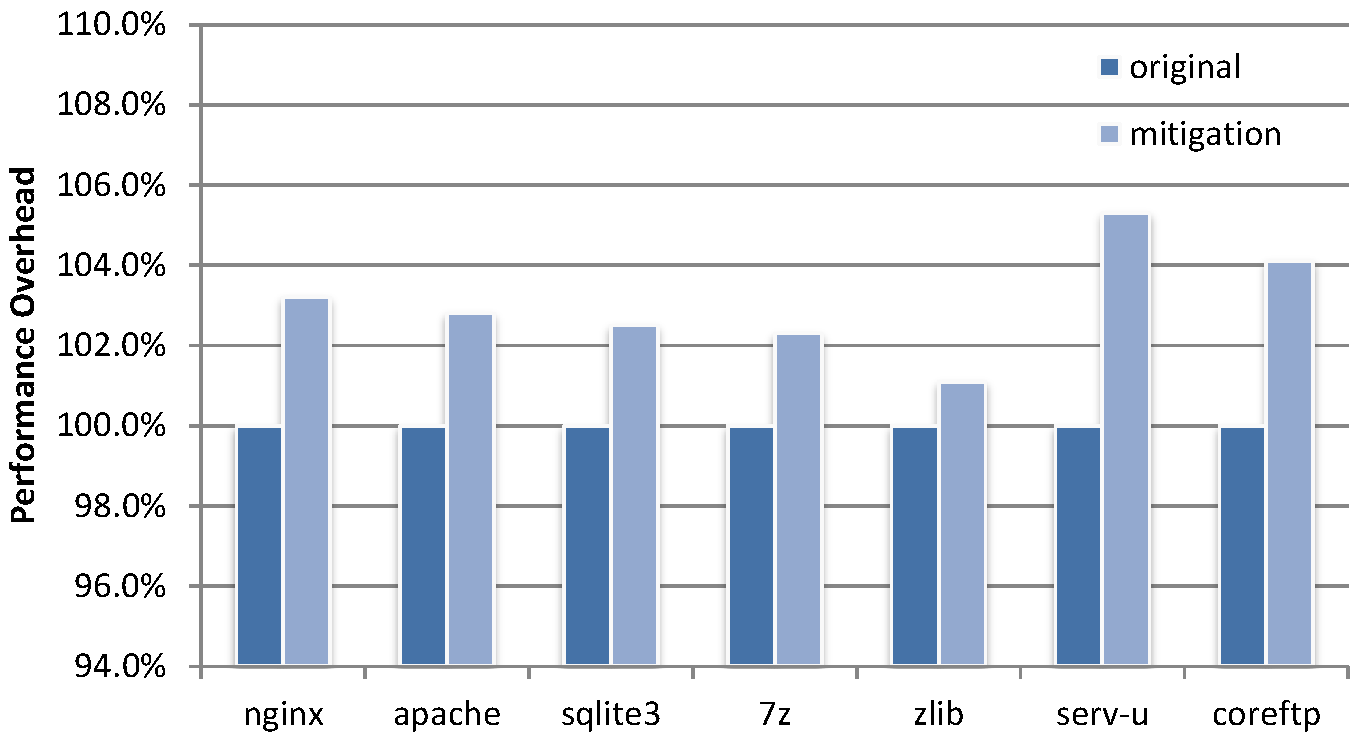
\includegraphics[width=0.47\textwidth]{figures/performance}
  \centering
  \caption{Performance overhead in non-trivial applications. Overhead mostly being introduced on system calls that need to fetch user-mode parameters}
  \label{fig:performance}
\end{figure}

~\autoref{fig:performance} shows the performance overhead of our mitigation in several non-trivial application. Some of those applications potentially could be the trampoline service of kernel TOCTOU attacks.
For web server software such as Nginx. We test its performance by counting the accumulated response time for 10000 web requests. For compression software such as zlib, we test it with compressing large files. For sqlite3, we use speedtest1.c which is a common performance testing program.

The result shows that the performance overhead is modest. Because only the system calls that have user-mode buffer as their parameters will trigger SMAP exceptions. 

%Therefore the programs that have more system calls tends to have a higher performance overhead. We also count the ratio of SMAP exceptions to total page fault exceptions of one process.

% This is not correct, most page fault are caused by SMAP, following is the test results for nginx
%g_PagefaultCount 1000, g_PagefaultSMAPCount 992
%g_PagefaultCount 2000, g_PagefaultSMAPCount 1986
%g_PagefaultCount 3000, g_PagefaultSMAPCount 2982
%g_PagefaultCount 4000, g_PagefaultSMAPCount 3981
%g_PagefaultCount 5000, g_PagefaultSMAPCount 4980
%g_PagefaultCount 6000, g_PagefaultSMAPCount 5979
%g_PagefaultCount 7000, g_PagefaultSMAPCount 6978
%g_PagefaultCount 8000, g_PagefaultSMAPCount 7974
%g_PagefaultCount 9000, g_PagefaultSMAPCount 8968


Part of the overhead is introduced because of the overall intercepting of page fault exceptions of the system. The page fault handler is called in high frequency. Our page fault hook currently is installed directly in the IDT table of each processor. Hence every page fault exception goes through our handler. Even though we let go in the every beginning if the current CR3 doesn't match the targeted ones, still there will be several extra instructions for each exception. Later we will use hypervisor to provide special IDT just for the targeted processes, only during which the page fault handler is intercepted.

%Although we use virtualization techniques, but the hypervisor we use is a very simple one. Unlike commercial virtualization solutions such as VMWare, Xen and Qemu+Kvm, ours doesn't emulate any hardware devices nor intercept further page mapping translate that between host and guest. Only several types of VM-Exit is inevitable such as control register accessing which we do need to handle it too.

\subsubsection{Real-world Vulnerabilities}

We write a poc(proof of concept) attacking program to test our mitigation against CVE-2008-2252. it triggers the vulnerability, introduce a memory buffer overflow. 

%We test it on the Windows XP sp3 system with the vulnerable win32k.sys file whose version is 5.1.2600.5512. Because SMAP only available at Intel 5th generation CPU (architecture code name Broadwell). Hard-disk controller which integrated in the CPU corresponded chipset doesn't support ATA mode anymore, and Windows XP system doesn't support AHCI mode, so it's difficult to install it on a modern PC. Our testing environment is established using a virtual machine. Particularly, VMWare Workstation 14 Player, emulated "Intel Core i5-6200U CPU (2 cores) with 1GB of RAM", option "Virtualize Intel VT-x/EPT or AMD-v/RVI" also enabled.

The attacking program has two threads. The main thread first allocate a page at virtual address 0, which later used as the parameter to be sent into the vulnerable system call. The reason to choose page zero is for bypassing the parameter validity checking in system call NtUserMessageCall. Next, right after creating another thread, it keeps calling the vulnerable function SendMessage (WM\_COPYDATA) with the malicious parameters in a loop, which eventually calls the vulnerable win32k function xxxInterSendMsgEx. The created thread then keep modifying the parameter at page zero, also in a loop, simultaneously.

\begin{figure}[th]
  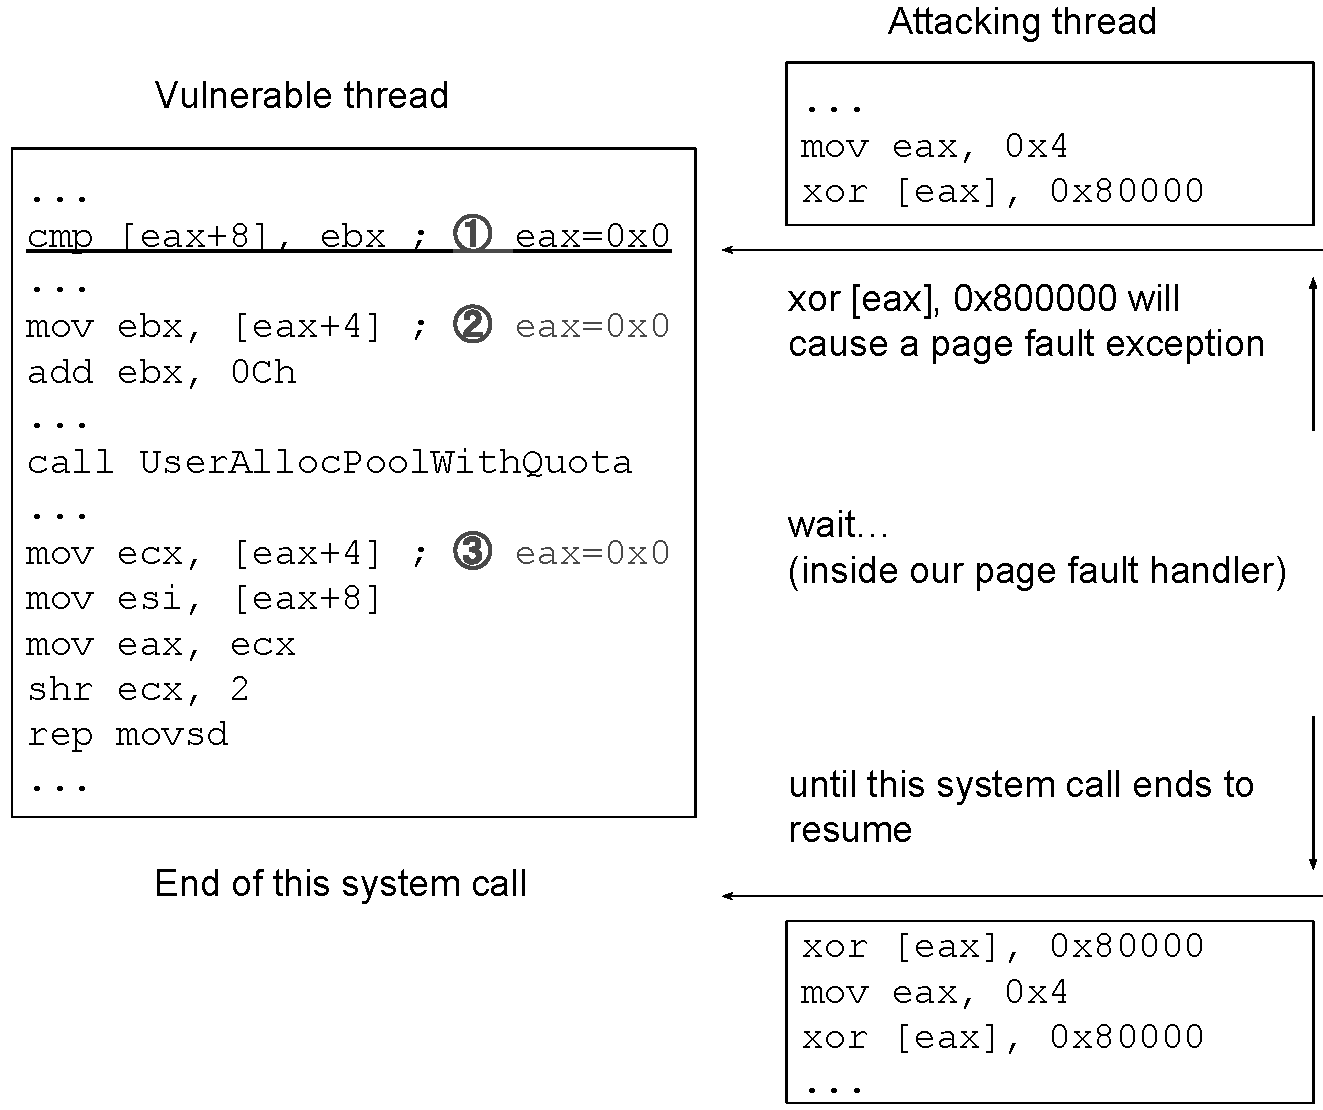
\includegraphics[width=0.47\textwidth]{figures/ms08061case}
  \centering
  \caption{The user page will be protected right at the moment it's been referenced.}
  \label{fig:ms08061case}
\end{figure}

In the attack, as shown in ~\autoref{fig:ms08061case}, the \textcircled{2} and \textcircled{3} are the places where vulnerable user-mode variable pcbData are referenced, it's address is 0x4. But the first time the zero page get accessed is \textcircled{1} where several instruction ahead of \textcircled{2}, it triggers an page fault exception (cased by SMAP). Therefore this page will be marked as a kernel page by our page fault handler. From this moment until the end of the current system call, this page will be protected from modifying by either as a kernel page or a user page with read-only permit. If the attacking thread try to modified it, another page fault exception  will be raised because of access violation. Then the attacking thread will be held for 30 milliseconds before it try to re-execute the faulting instruction again, for as many as 10 times. If not possible, the attacking thread will be terminated. We can see that during the protection, memory reads at \textcircled{2} and \textcircled{3} are kept consistent.


CVE-2013-1254 is another typical TOCTOU vulnerability that found in Windows win32k module~\cite{jurczyk2013identifying}. It effects both Windows XP and Windows 7. 

%A series of same kind of vulnerability found in 26 functions of module win32k.

\begin{lstlisting}[basicstyle=\small,style=redkeyword] 
.text:BF8A993F   mov   eax, _W32UserProbeAddr
                       .
                       .
.text:BF8A9973   @cmp   [ecx+8], eax@    
.text:BF8A9976   jnb   short loc_BF8A997B
.text:BF8A9978   @mov   eax, [ecx+8]@    
.text:BF8A997B
.text:BF8A997B loc_BF8A997B:                           
.text:BF8A997B   mov   ecx, [eax]
.text:BF8A997D   mov   eax, [eax+4]
\end{lstlisting}
%\captionof{lstlisting}{Flawed code in win32k.sys function SfnINOUTSTYLECHANGE()}

The flawed function first fetch a value from \[ecx+8\] and compare it with \_W32UserProbeAddress which is a value that indicates the highest possible address for user-mode variables. It confirms that the variable is actually reside in user space. Next, it fetches the value again and assign it to eax. This is where the double fetch happens. The attacker can change the value between those two fetches, letting it bypass the verification,  then assign it a kernel space address.

So when \[ecx+8\] is referenced the first time, the corresponding page will trigger a SMAP exception, then this page will be protected until the current system call ends. Other threads write to it will also trigger page fault exceptions, as explained in the previous case, out page fault handler will handle those to keep the data consistent. 


